\section{Lattice: lattice definition, base of a lattice, CVP problem, SVP problem, Hadamard ratio, Babai algorithm, GGH public key cryptosystem.}

\newcommand{\lat}{\ensuremath{\mathcal{L}}}
\newcommand{\base}{\ensuremath{\text{\textbf{B}}}}

Mřížka je sada bodů v~n-dimenzionálním prostoru s~periodickou strukturou.
V~rovině ji lze popsat kartézskými souřadnicemi $(x, y)$.
Mřížky se definují jejich bázovými vektory:
$$\lat = \lat(b_1, b_2) = \{x_1b_1 + x_2b_2 : x_i \in \mathbb{Z}\}$$

N-dimenzionální mřížka $\lat$ je množina všech celočíselných kombinaí n-lineárně nezávislých vektorů (generátorů)
$$b_1, \dots, b_n \in \mathbb{R}^n : \lat = \left\{\sum_{i=1}^n x_ib_i : x_i \in \mathbb{Z}\right\}$$

$\mathcal{B} = \{b_1, \dots, b_n\}$ se nazývá bází mřížky.
Platí že každý vektor $v \in \lat$ může být unikátně vyjářden jako lineární kombinace bázových vektorů: $v = a_1b_1 + \cdots + a_nb_n$.

V~kryptografii se využívají mřížky splňující podmínku $q \mathbb{Z}^n \subset \lat \subset \mathbb{Z}^n$ pro~některé (prvočíselné)~$q$.
Jako matice se využívá
$\base = \left( \begin{matrix}
| & | & {} & | \\
b_1 & b_2 & \cdots & b_n \\
| & | & {} & |
\end{matrix} \right);\ \lat(\base) = \{\base x : x \in \mathbb{Z}^n\}$:
například mřížka s~bázovými vektory
$b_1 = (3, 2)$, $b_2 = (1, 3)$
je zapsána jako
$\lat(\base) = \left\{\left(\begin{matrix}3&1\\2&3\end{matrix}\right)\left(\begin{matrix}x_1\\x_2\end{matrix}\right): x_1, x_2 \in \mathbb{Z}\right\}$.


\subsection{Báze mřížky}

Báze není unikátní; jedna mřížka má nekonečně mnoho kombinací bázových vektorů.

\underline{Dobrá báze} je jednoduchá na výpočty, naopak se \underline{špatnou bází} jsou výpočty komplikované a některé~problémy jsou v~nich neřešitelné; proto se dobrá báze používá jako privátní číslo a špatná báze jako veřejné číslo.
Dobré báze je blízká bázi ortogonální.

% TODO Používá se 'unimodulární' i v češtině?
Mezi bázemi je možné (jednosměrně) převádět násobením unimodulární\footnotemark{} maticí $U$.
\footnotetext{Matice je unimodulární tehdy pokud je její determinant $\pm 1$.}

\subsection{Hadamardův poměr}

Platí
$
\mathcal{H} =
\left( \frac{
| \text{det} \, \lat(v_1, \dots, v_n) | }{
|| v_1 ||_2 \cdot || v_2 ||_2 \cdot \dots \cdot ||v_n||_2
} \right)^{\frac{1}{n}}
$.
Dobrá báze má $\mathcal{H}$ blízko jedné.

% TODO Blíže vysvětlit co přesně znamená jmenovatel.
% TODO Jak vypadají špatné báze? Napsat jaké hodnoty mohou mít -- větší nebo menší?


\subsection{CVP, SVP}

\textbf{\emph{Shortest Vector Problem}}: pro~zadanou mřížku $\lat$ najděte nejkratší nenulový vektor $v$ z~$\lat$ s~minimální velikostí $||v||_2$.
V~současnosti neexistuje žádný algoritmus s~polynomiální složitostí.
Existují deterministické ($n^{O(n)}$)\footnotemark{} či randomizované ($2^{O(n)}$)\footnotemark{}; rychlejší nejsou pravděpodobné, protože jde o~NP-hard problém.
\footnotetext{Kannan, Ravi (1983): Improved Algorithms for Integer Programming and Related Lattice Problems \\ \url{https://doi.org/10.1145/800061.808749}}
\footnotetext{Ajtai, Miklós; Kumar, Ravi; Sivakumar, D. (2001): A sieve algorithm for the shortest lattice vector problem \\ \url{https://doi.org/10.1145/380752.380857}}

\emph{Worst-case} SVP je možné redukovat na~\emph{average-case}\footnotemark{}.
\footnotetext{Ajtai, Miklós (1998): The shortest vector problem in L2 is NP-hard for randomized reductions. \\ \url{https://doi.org/10.1145/276698.276705}}
Nejde o~problém dostatečně složitý pro~praktickou kryptografii.

\textbf{\emph{Closest Vector Problem}}: pro~zadanou mřížku $\lat$ a vektor $t \in \mathbb{R}^n$ najděte nenulový vektor $v \in \lat$ takový abyste minimalizovali $||t - v||_2$.
Existuje deterministický algoritmus ($n^{O(n)}$)\footnotemark{}.
\footnotetext{Micciancio, Daniele; Voulgaris, Panagiotis (2010): Faster Exponential Time Algorithms for the Shortest Vector Problem \\ \url{https://doi.org/10.1137/1.9781611973075.119}}

Jinými slovy jde o~prohledávání okolí vektoru a~nalezení bázového vektoru který je k~hledanému nejbližší.
Jde o~generalizaci SVP.
CVP$_\gamma$: vzdálenost může být nejvýše $\gamma$.
Platí že $\gamma$-GapCVP' je NP-hard pro~$\gamma \ge 1$\footnotemark{}.
\footnotetext{Arora, S., L. Babai, J. Stern, and E.Z. Sweedyk (1997). The hardness of approximate optima in lattices, codes, and systems of linear equations}


\subsection{Babaiův algoritmus}

Pokud je $\base$ ortogonální báze v~$\lat$, approx-CVP může být vyřešen v~polynomiálním čase.
Algoritmus funguje i při~dostatečně ortogonálních bázích.

\begin{enumerate}
\item $t = t_1 b_1 + t_2 b_2 + \cdots + t_n b_n$ kde $t_1, t_2, \dots, t_n \in \mathbb{R}$.
\item $v = a_1 b_1 + a_2 b_2 + \cdots + a_n b_n$ kde $a_i = \lceil t_i \rfloor$ pro $i = 1, 2, \dots, n$.
\end{enumerate}

% FIXME Vysvětlení?

\begin{figure}[ht]
    \emph{Příklad}: Pro $t = (-1.1, 6.2)$ získejte $v$.

    \begin{minipage}{0.5\textwidth}
        \centering
        \caption*{\emph{dobrá báze:}}

        $b_1 = (5, 0)$, $b_2 = (1, 2)$

        $t_1\left(\begin{matrix}5\\0\end{matrix}\right) + t_2 \left(\begin{matrix}1\\2\end{matrix}\right) = \left(\begin{matrix}-1.1\\6.2\end{matrix}\right)$

        $v = -b_1 + 3b_2 = (-2, 6)$
    \end{minipage}\hfill\begin{minipage}{0.5\textwidth}
        \centering
        \caption*{\emph{špatná báze:}}

        $b_1 = (9, 8)$, $b_2 = (8, 6)$

        $t_1\left(\begin{matrix}9\\8\end{matrix}\right) + t_2 \left(\begin{matrix}8\\6\end{matrix}\right) = \left(\begin{matrix}-1.1\\6.2\end{matrix}\right)$

        $v = 6b_1 - 7b_2 = (6, 12)$
    \end{minipage}
\end{figure}


\subsection{Asymetrický kryptosystém GGH}

Alice vybírá lineárně nezávislé vektory $v_1, v_2, \dots, v_n \in \mathbb{Z}^n$ které jsou k~sobě celkem kolmé (což lze zjistit Hadamardovým poměrem).
Vektory $v_i$ jsou Alicin privátní klíč (uspořádán do~řádků v~$n \times n$ matici $V$).

Alice vytvoří $n \times n$ matici $\textbf{U}$ tak aby $\text{det}(\textbf{U}) = \pm 1$.
Poté spočítá $\textbf{W} = \textbf{UV}$.
Řádky matice $\textbf{W}$ ($w_1, \dots, w_n$) je nová báze $\lat$ a Alicin veřejný klíč.

Pro~poslání zprávy vybere Bob malý vektor $m$ s~celočíselnými souřadnicemi.
Vybere také náhodný rušivý vektor $r$ (např. z~předem definovaného rozsahu $-\delta$ až $\delta$) a vypočítá
$e = m\textbf{W} + r = \sum_{i=1}^n m_i w_i + r_i$.

Alice použije Babaiův algoritmus se~svou dobrou bází $v_1, \dots, v_n$ k~nalezení vektoru v~$\lat$ blízkému $e$.
Protože používá dobrou bázi a~$r$ je malé, vypočítá $m\textbf{W}$.
Tuto hodnotu vynásobí $\textbf{W}^{-1}$ a tím získá $m$.

Jde o~schéma bezpečné, ale kvůli velikosti bezpečnostních parametrů nepraktické.
(Převzato z~\emph{An Introduction to Mathematical Cryptography}\footnotemark{}).
\footnotetext{\url{https://staff.emu.edu.tr/alexanderchefranov/Documents/CMSE491/CMSE491 Fall2020/Hoffstein2015 Introduction to Mathematical Cryptography 409-412 GGH.pdf}. \\ Plně dostupné na \url{https://doi.org/10.1007/978-1-4939-1711-2}}


\clearpage
\section{LWE and RLWE: LWE problem, RLWE problem, Regev one-bit cryptosystem.}

Všechny LWE problémy jsou do~určité míry ekvivalentní (pro~rovnou bezpečnost může být nutné upravit bezpečnostní parametry).
V~praxi proti nim neexistuje útok.

Obecně jde o~řešení problému soustavy rovnic.
Samotná matice lze řešit Gaussovskou eliminací, ale po~přidání chyby $e \in \{-1, 0, 1\}$ k~výsledkům již správný výsledek vycházet nebude.

$$
\left[
\begin{matrix}
1 & 5 & 3 & 2 \\
1 & 4 & 2 & 6 \\
2 & 1 & 3 & 1 \\
3 & 4 & 4 & 6 \\
\end{matrix}
\right] \equiv \left[
\begin{matrix}
1 \\ 2 \\ 4 \\ 0
\end{matrix}
\right] \mod 7
\hspace*{2em}
\equiv \left[
\begin{matrix}
1+1=2 \\ 2+0=2 \\ 4-1=3 \\ 0-1=6 \\
\end{matrix}
\right] \mod 7
$$


\subsection{Learning with Errors}

LWE lze zapsat jako $\textbf{A}s + e = b$. Obsahuje $n$ polynomů (řádu $m$), tajemství $s$ a chybu $e$.

$s$ je nalezitelné linearizací pokud je $\chi$ náhodně rozložené v~$\mathbb{Z}_2$ (tj. $n=1$ a $e \in \{-1, 0, 1\}$).
Bezpečnost tedy závisí na~volbě distribuce $\chi$.

Je možné ho uplatit na~symetrické i asymetrické šifrování, výměnu klíčů, digitální podpisy, (plně) homomorfní šifrování, ZK protokoly a další.

\subsection{Ring Learninig with Errors}

LWE trpí velikostmi klíčů ($n^2$).
R-LWE redukuje matici \textbf{A} na~jediný řádek, který je pokaždé horizontálně posunutý o~jednu pozici vpravo.
Stačí tak přenášet pouze tento jeden řádek a ne~celou matici.
Vytvořená struktura je ideální mřížka, ve~které může být grupa $\mathbb{Z}_q^n$ nahrazena polynomiálním okruhem $\mathbb{Z}_q[x]/\left<x^n+1\right>$.

R-LWE lze zapsat jako $\textbf{A} + s \equiv b$. Obsahuje $n$ polynomů (řádu $m$) a tajemství $s$.

Redukce na~polynomy výrazně zmenšuje velikost přenášených klíčů $\textbf{A}, s$.

\subsection{Regev one-bit kryptosystém}

\begin{wrapfigure}{r}{16em}
    \centering
    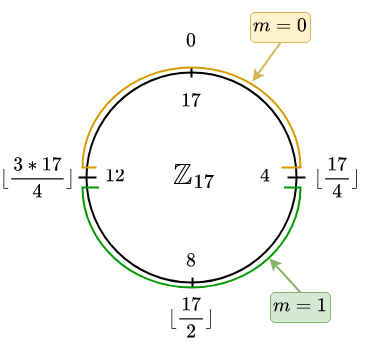
\includegraphics[width=13em]{regev}
\end{wrapfigure}

Schéma stavící na~LWE.
Privátním klíčem je $s$, $e$, veřejným $A$, $b$.

Chceme zašifrovat jednobitovou zprávu $m$.
V~určité grupě ($\mathbb{Z}_{17}$) můžeme zvolit $p$ takové aby $c = p+m$ šumem nepřerušilo zprávu.

V~našem konkrétním případě $\mathbb{Z}_{17}$ může být šum maximálně $\pm \frac{17}{4}$.
Dešifrováno bude $\begin{cases}
1: & p \in \left<5, 11\right> \\
0: & p \in \left<-4, 3\right> \\
\end{cases}$.

% NOTE Zde je možné přidat schéma/obrázek z prezentace (Post-Quantum Cycles, slide 28)


\clearpage
\section{Lattice-based protocols: Module-LWE problem, LWR problem, NTT, KYBER scheme, SABER scheme.}

\clearpage
\section{Homomorphic Encryption (HE): homomorphism, HE definition, kind of HE (partially, somewhat, fully), Bootstrapping, Paillier Cyrptosystem}

\clearpage
\section{Secret Sharing: Threshold Secret Sharing, Shamir Secret Sharing, unique polynomial theorem, Interpolation problem.}

\clearpage
\section{Secure Multi-Party Computation (SMPC): SMPC definition, SMPC security requirement and adversarial behavior, e-voting, oblivious transfer}

\clearpage
\section{Blockchain and Smart Contracts: blockchain architecture, transactions and blocks, mining, forks, consensus, smart contracts, 51 \% attack on blockchain.}

\clearpage
\section{Cryptocurrencies: cryptocurrency (definition, requirements), Ecash, Bitcoin, CryptoNote, proof of work in Bitcoin, Bitcoin address and wallet, Bitcoin’s transaction flow, double spending problem.}

\clearpage
\section{Data privacy 1: statistical disclosure control methods, disclosure risk, information loss, microdata, privacy categories (identifiers, quasi-identifiers, sensitive data), non-perturbative methods (sampling, global recording, suppression)}

\clearpage
\section{Data privacy 2: syntethic data, perturbative masking (noise addition, microaggregation, rank swapping), k-anonymity, record linkage}
